\documentclass[conference]{IEEEtran}

% ========= 日本語対応(LuaLaTeX推奨) =========
\usepackage{luatexja}
\usepackage{luatexja-fontspec}
% HaranoAjiフォント(TeX Live 標準)
\setmainjfont{HaranoAjiMincho}
\setsansjfont{HaranoAjiGothic}

% ========= 一般パッケージ =========
\usepackage{amsmath,amssymb}
\usepackage{graphicx}
\usepackage{booktabs}
\usepackage{array}        % p{..}列幅の表で安定
\usepackage{url}
\usepackage[hidelinks]{hyperref}
\usepackage{cite}

% ========= 図・グラフ =========
\usepackage{tikz}
\usetikzlibrary{arrows.meta,decorations.pathreplacing,calc,patterns}
\usepackage{pgfplots}
\pgfplotsset{compat=1.17} % 1.18でもOKなら上げてよい

% ========= 浮動体の制御(ページ数減少・配置失敗の抑制)=========
\usepackage{stfloats}          % IEEEtranとの相性良。bottom配置など柔軟化
\usepackage[section]{placeins} % セクション跨ぎの飛び過ぎを防止(\FloatBarrier)
\makeatletter
\def\fps@figure{tbp}           % [t]固定で詰まるのを回避
\def\fps@table{tbp}
\makeatother

% ========= タイトル =========
\title{DRAM技術導入とその戦略的位置づけ(1997--2001)\\
\large 酒田FabにおけるDRAM/PSRAMとロジック展開の連関}

% ========= 著者情報 =========
\author{%
  \IEEEauthorblockN{三溝 真一 (Shinichi Samizo)}%
  \IEEEauthorblockA{独立系半導体研究者(元セイコーエプソン)\\%
  Independent Semiconductor Researcher (ex-Seiko Epson)\\%
  Email: \href{mailto:shin3t72@gmail.com}{shin3t72@gmail.com}\\%
  GitHub: \url{https://github.com/Samizo-AITL}}%
}

\begin{document}
\maketitle

\begin{abstract}
本論文は,1997年から2001年にかけてセイコーエプソン酒田事業所が
三菱電機からの技術移管を通じて \mbox{0.5\,$\mu$m} $\rightarrow$ \mbox{0.35\,$\mu$m} $\rightarrow$ \mbox{0.25\,$\mu$m} の
DRAMプロセスを短期間で習得し,得られたプロセス知見を
先端ロジックおよび高耐圧混載CMOSへ展開して液晶ドライバー製品化に結びつけた
技術的・戦略的過程を,筆者の実体験に基づき整理する。
主要な不良モード(Pause/Disturb Refresh)の物理起源と対策,
および量産歩留まりの推移を示し,獲得した知見がその後の
事業ドメインへどのように接続されたかを考察する。
\end{abstract}

\begin{IEEEkeywords}
DRAM,VSRAM/PSRAM,0.25\,$\mu$mプロセス,リテンション不良,ディスターブ不良,
酒田Fab,技術移管,高耐圧混載CMOS,液晶ドライバー,プロセス習得
\end{IEEEkeywords}

\section{序論}
1997年,当時の半導体産業は Windows~95 の普及や 8インチラインの量産普及により急伸した。
セイコーエプソンは酒田事業所(8インチFab)において,
三菱電機からの技術移管により 0.5\,$\mu$m $\rightarrow$ 0.35\,$\mu$m $\rightarrow$ 0.25\,$\mu$m
のDRAM三世代を短期間で習得した。
狙いはDRAMで勝つこと自体ではなく,DRAMを媒体に先端プロセスを自前化し,
最終的にロジック/高耐圧混載CMOS(液晶ドライバー等)で差別化することにあった。
本稿はその実践知を,立ち上げの不良モード解析・対策・歩留まり推移とともに記録する。

\section{第1章:0.5\,\texorpdfstring{$\mu$m}{μm} と 0.35\,\texorpdfstring{$\mu$m}{μm} 世代の立ち上げ}

\subsection{0.5\,$\mu$m 16M DRAM}
酒田Fabにおける最初の量産製品は 0.5\,$\mu$m世代の16M DRAM であった。
熊本Fabで確立済みのプロセスを導入し,設備親和性も高く,初期から安定した歩留まりで量産に到達した。
これにより酒田Fabが量産可能な生産拠点であることを内外に示せた。

\subsection{0.35\,$\mu$m 64M DRAM:洗浄フロー差異と「鏡写し」}
1997年秋,0.35\,$\mu$m世代 64M DRAM の試作で 30ロット超連続の形状不良が発生。
熊本では安定のプロセスが酒田で再現できなかった。
徹底調査の結果,原因は \emph{洗浄フローの差異} であった。
熊本:硫酸過水 $\rightarrow$ アンモニア過水 $\rightarrow$ 塩酸過水,
酒田:工程短縮で硫酸過水を省略(アンモニア過水 $\rightarrow$ 塩酸過水)。
表面状態の差が後工程プラズマ処理と相互作用し膜厚ばらつき・形状崩れを誘発。
最終対応は熊本プロセスの完全な \emph{鏡写し}(フロー・装置条件・手順すべて)であり,
これにより量産に成功した。
この経験は「先端移管で一切の省略を許さない」というFabの共通認識を形成した。

\subsection{小括}
0.5\,$\mu$mは円滑に量産化,0.35\,$\mu$mは洗浄省略が致命要因で,
完全鏡写しで回復。以降世代への重要教訓となった。

\FloatBarrier

\section{第2章:0.25\,\texorpdfstring{$\mu$m}{μm} 世代64M DRAMの立ち上げ}

\subsection{SCF方式と初期歩留まり}
1998年,酒田Fabは 0.25\,$\mu$m世代64M DRAM に挑戦した。
立ち上げ方式は \emph{Short Cycle Feedback (SCF)} を継続採用(0.5\,$\mu$m時からの三菱方式)。
短サイクルで評価・フィードバックを回し工程最適化を加速し,
初期本番ロットで歩留まり約 65\% を達成した。
一般に新世代DRAM初期は20–30\%からのスタートが多く,65\%は高い水準といえる。

手順: (1) フロッピー2枚の移管条件を流動票へ展開,
(2) 主要工程で形式ロット(約10)を途中止め観察,
(3) SEM・電気評価で条件修正,(4) 本番ロット(3)を全工程流し長期信頼性確認。

\subsection{保持時間モデルと不良モード解析}
初期不良は \emph{Pause Refresh Fail} に集中。
32\,ms $\rightarrow$ 64\,ms $\rightarrow$ 128\,ms と停止時間を伸ばすと単ビット不良が散発増加。
ライン欠陥・エッジ集中はなく全体にランダム(Fig.~\ref{fig:failmap})。
保持時間は
\begin{equation}
\tau = \frac{C_{\mathrm{cell}} \cdot V_{\mathrm{cell}}}{I_{\mathrm{leak}}}
\end{equation}
で表され,$C_{\mathrm{cell}}$ と $V_{\mathrm{cell}}$ は設計通り。
主因は \emph{拡散層ジャンクションリーク} 増大であると特定。
同一座標での再現も確認され,プロセス起因の系統要因が示唆された(Fig.~\ref{fig:dram_cross_section})。

% ---- 断面図(1カラム確実化) ----
\begin{figure}[t]
\centering
\resizebox{\columnwidth}{!}{%
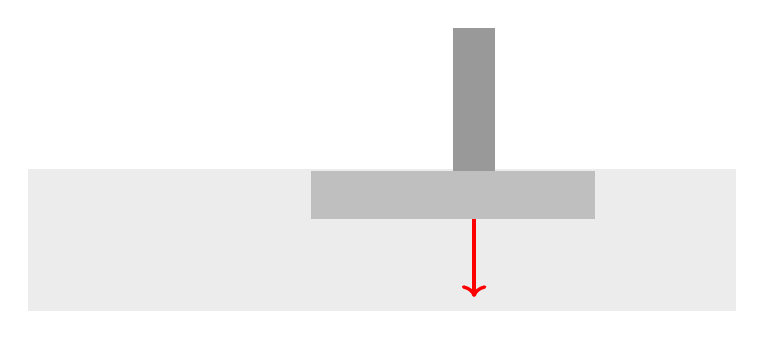
\begin{tikzpicture}[scale=1.8]
  % p- substrate
  \fill[gray!15] (-1,0) rectangle (4,-1.0);
  % n+ diffusion
  \fill[gray!50] (1,-0.01) rectangle (3,-0.35);
  % Storage Node Contact (filled, no stroke)
  \fill[black!40] (2,-0.01) rectangle (2.3,1.0);
  % leakage arrow
  \draw[->,very thick,red] (2.15,-0.35) -- (2.15,-0.9);
\end{tikzpicture}
}
\caption{DRAM セル断面概念図(SNコンタクト/$n^+$拡散層/$p^-$基板)。赤矢印は $n^+ \rightarrow p^-$ のリーク $I_{\mathrm{leak}}$。}
\label{fig:dram_cross_section}
\end{figure}

% ---- ウエハ・フェイルマップ(1カラム確実化) ----
\begin{figure}[t]
\centering
\resizebox{\columnwidth}{!}{%
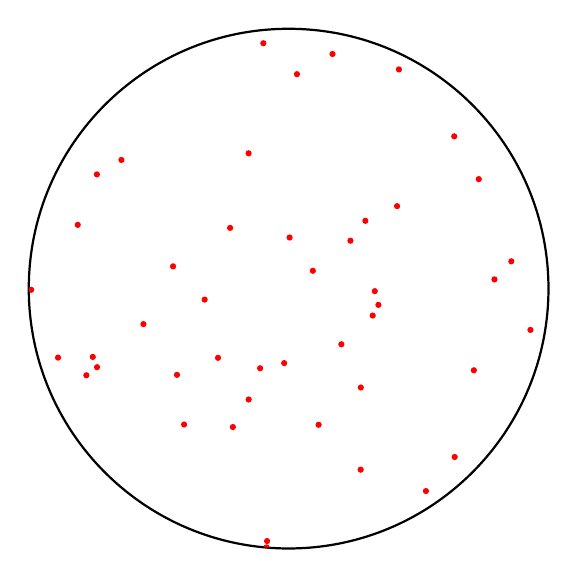
\begin{tikzpicture}[scale=0.22]
  \def\R{15}
  \draw[thick] (0,0) circle (\R);
  \begin{scope}
    \clip (0,0) circle (\R);
    \foreach \i in {1,...,60}{
      \pgfmathsetmacro{\xx}{(rnd*2-1)*\R}
      \pgfmathsetmacro{\yy}{(rnd*2-1)*\R}
      \fill[red] (\xx,\yy) circle (0.18);
    }
  \end{scope}
\end{tikzpicture}
}
\caption{Pause Refresh Fail のフェイルビットマップ例(ウエハ外周円+ランダム赤点)。}
\label{fig:failmap}
\end{figure}

\subsection{プラズマダメージ仮説}
ジャンクションリーク増大の要因として \emph{プラズマダメージ} を疑った。
ゲートエッチ後の酸化膜露出時や LDD 工程での繰り返しアッシングで界面欠陥準位が形成され,
熱励起キャリア生成を介してリークが増えると推定。

\subsection{対策と効果}
根本対策は \emph{レジスト剥離の全面切り替え}:
O$_2$アッシング(ドライ剥離)から \emph{硫酸剥離}(ウエット剥離)へ。
感受性の高い工程後のプラズマ曝露を \emph{ゼロ化} し,
界面欠陥・ジャンクションリークの生成を根本抑制した
(アッシング低パワー化は実施せず,フローを変更)。

\begin{table}[t]
  \centering
  \caption{レジスト剥離フローの切替(Before/After)}
  \label{tab:resist_flow}
  \begin{tabular}{p{0.25\linewidth} p{0.65\linewidth}}
    \toprule
    従来(Before) & O$_2$アッシングによるドライ剥離 \\
    対策後(After) & 硫酸剥離によるウエット剥離 \\
    主効果 & プラズマ曝露ゼロ化,界面欠陥・ジャンクションリーク抑制 \\
    歩留まり & 65\% $\rightarrow$ 80\%台後半(Pause改善が支配) \\
    \bottomrule
  \end{tabular}
\end{table}

この切替により Pause は大幅減,量産歩留まりは 65\% $\rightarrow$ 80\%台後半へ改善(Fig.~\ref{fig:yield_trend})。

% ---- 歩留まりトレンド(1カラム) ----
\begin{figure}[t]
\centering
\begin{tikzpicture}
\begin{axis}[
  width=\columnwidth,
  height=6cm,
  ymin=0, ymax=100,
  ylabel={歩留まり(\%)},
  symbolic x coords={0.5\,\mu m,0.35\,\mu m,0.25\,\mu m,VSRAM},
  xtick=data, xlabel={プロセス世代},
  grid=both,
  legend style={at={(0.5,-0.28)},anchor=north,draw=none,fill=none,font=\footnotesize},
  legend columns=2,
  clip=false
]
  \addplot+[semithick,mark=*]
    coordinates {(0.5\,\mu m,95) (0.35\,\mu m,20) (0.25\,\mu m,65) (VSRAM,30)};
  \addlegendentry{初期歩留まり}
  \addplot+[semithick,mark=square*]
    coordinates {(0.5\,\mu m,95) (0.35\,\mu m,86) (0.25\,\mu m,88) (VSRAM,80)};
  \addlegendentry{改善後}
\end{axis}
\end{tikzpicture}
\caption{酒田Fabにおける世代別歩留まり推移。}
\label{fig:yield_trend}
\end{figure}

\subsection{小括}
SCFで迅速に条件整備し初期65\%を確保。主因はジャンクションリークで,
ウエット剥離(硫酸剥離)への切替で 80\%台後半へ改善。
表面処理・プラズマ影響の軽視が致命的になり得ることを教訓化した。

\FloatBarrier

\section{第3章:VSRAM(2001年)— Pause/Disturb対策と歩留まり改善}

\subsection{開発背景と初期状況}
世界初のカメラ付き携帯の実現に向け,低消費・高温(90$^\circ$C)保証が必須。
0.25\,$\mu$m DRAMプロセス流用+内部リフレッシュ制御で \emph{VSRAM} を立ち上げたが,
初期量産歩留まりは約30\%。筆者は改善を担当。

\subsection{顕在化した不良モード}
\textbf{Pause}:リフレッシュ停止で保持不足。  
\textbf{Disturb}:リフレッシュ中のワードライン電圧が隣接セルに影響し誤反転。

\subsection{物理的要因}
Pause の主因はセル \emph{ジャンクションリーク}。
温度上昇で指数的に増大し,バックバイアス強化で抑制可能(Fig.~\ref{fig:pause_temp_junc})。
Disturb は \emph{短チャネル効果(SCE)} によるオフリーク増大が支配的で,高温で顕著(Fig.~\ref{fig:disturb_temp_sce})。

% ---- Pause(温度×Vbs) ----
\begin{figure}[t]
\centering
\begin{tikzpicture}
\begin{axis}[
  width=\columnwidth, height=6cm,
  xlabel={温度 [$^\circ$C]}, ylabel={ジャンクションリーク $I_{\mathrm{junc}}$(相対)},
  ymode=log, ymin=1e-2, ymax=1e2,
  xmin=25, xmax=100, xtick={25,40,60,80,90,100},
  grid=both,
  legend style={at={(0.5,-0.22)},anchor=north,draw=none,fill=none},
  clip=false
]
  \addplot+[semithick,mark=*] coordinates {
    (25,0.02) (40,0.06) (60,0.3) (80,1.6) (90,3.2) (100,6.0)
  };
  \addlegendentry{$V_{bs}=-1$\,V}
  \addplot+[semithick,mark=square*] coordinates {
    (25,0.01) (40,0.03) (60,0.12) (80,0.45) (90,0.9) (100,1.8)
  };
  \addlegendentry{$V_{bs}=-3$\,V}
\end{axis}
\end{tikzpicture}
\caption{Pause:温度上昇で $I_{\mathrm{junc}}$ は指数的に増大。バックバイアス強化で抑制。}
\label{fig:pause_temp_junc}
\end{figure}

% ---- Disturb(温度×CD) ----
\begin{figure}[t]
\centering
\begin{tikzpicture}
\begin{axis}[
  width=\columnwidth, height=6cm,
  xlabel={温度 [$^\circ$C]}, ylabel={トランジスタリーク $I_{\mathrm{off}}$(相対)},
  ymode=log, ymin=1e-3, ymax=1e1,
  xmin=25, xmax=100, xtick={25,40,60,80,90,100},
  grid=both,
  legend style={at={(0.5,-0.22)},anchor=north,draw=none,fill=none},
  clip=false
]
  \addplot+[semithick,mark=triangle*] coordinates {
    (25,0.004) (40,0.01) (60,0.05) (80,0.22) (90,0.45) (100,0.9)
  };
  \addlegendentry{CD=0.25\,$\mu$m}
  \addplot+[semithick,mark=*] coordinates {
    (25,0.01) (40,0.03) (60,0.15) (80,0.7) (90,1.4) (100,2.8)
  };
  \addlegendentry{CD=0.20\,$\mu$m}
\end{axis}
\end{tikzpicture}
\caption{Disturb:短チャネル化で $I_{\mathrm{off}}$ が増大。温度上昇でも指数増。}
\label{fig:disturb_temp_sce}
\end{figure}

\subsection{対策と実装}
\textbf{Pause対策}:HF洗浄回数最小化(ゲート酸化膜残膜を確保し SN近傍リーク低減),
バックバイアス強化($V_{bs}=-1\to -3$ V)。  
\textbf{Disturb対策}:ゲートCD中心値の厳密管理,バックバイアス強化で $V_{\mathrm{th}}$ を上げ誤反転を抑制,
メモリセルのチャネルドーピング量を動作可能範囲で増やし $V_{\mathrm{th}}$ を底上げ。

\begin{table}[t]
\centering
\caption{Pause / Disturb 不良に対する主な対策}
\label{tab:pd_measures}
\begin{tabular}{p{0.18\linewidth} p{0.28\linewidth} p{0.46\linewidth}}
\toprule
不良モード & 主因 & 主な対策 \\
\midrule
Pause   & ジャンクションリーク 
        & HF洗浄制御,バックバイアス強化 \\
Disturb & 短チャネル効果 
        & CD管理,チャネルドーピング,バックバイアス強化 \\
\bottomrule
\end{tabular}
\end{table}

\subsection{効果と歩留まり}
Pause/Disturb の双方が改善し,歩留まりは 30\% $\rightarrow$ 80\%台に到達。

\FloatBarrier

\section{第4章:0.18\,\texorpdfstring{$\mu$m}{μm} トレンチ系の評価と断念}
\subsection{評価対象と背景}
VSRAMの次世代候補として,NANYA 0.18\,$\mu$m(東芝系)のトレンチDRAMプロセスを評価。
面積効率は高いが,ジャンクション面積拡大でリークが増えやすい。

\subsection{課題の顕在化}
90$^\circ$C 条件で Pause/Disturb が顕著化。ジャンクション面積に比例して $I_{\mathrm{junc}}$ が増加し,
高温ほど増加率が大(Fig.~\ref{fig:trench_area_leak})。

% ---- トレンチ面積×リーク ----
\begin{figure}[t]
\centering
\begin{tikzpicture}
\begin{axis}[
  width=\columnwidth, height=6cm,
  xlabel={ジャンクション面積(相対)}, ylabel={ジャンクションリーク $I_{\mathrm{junc}}$(相対)},
  xmin=0.5, xmax=2.5, ymin=0, ymax=3.5,
  xtick={0.5,1.0,1.5,2.0,2.5},
  ytick={0,0.5,1.0,1.5,2.0,2.5,3.0},
  grid=both,
  legend style={at={(0.5,-0.22)},anchor=north,draw=none,fill=none},
  clip=false
]
  \addplot+[semithick,mark=square*] coordinates {
    (0.5,0.25) (1.0,0.5) (1.5,0.8) (2.0,1.1) (2.5,1.4)
  };
  \addlegendentry{80$^\circ$C}
  \addplot+[semithick,mark=*] coordinates {
    (0.5,0.5) (1.0,1.0) (1.5,1.6) (2.0,2.2) (2.5,2.9)
  };
  \addlegendentry{90$^\circ$C}
\end{axis}
\end{tikzpicture}
\caption{トレンチキャパ:面積に比例して $I_{\mathrm{junc}}$ が増加。高温ほど増加率が大。}
\label{fig:trench_area_leak}
\end{figure}

\subsection{評価結果と戦略判断}
NANYA 0.18\,$\mu$m は 90$^\circ$C 動作保証に難があり,次世代VSRAMは断念。
一方で液晶ドライバーICへの集中(高耐圧混載CMOS)が戦略として明確化した。

\subsection{小括}
汎用DRAM技術のモバイル適用限界を確認。得られた知見は
高耐圧・混載技術(液晶ドライバー)へ直結し,事業の主戦場を転換。

\section{結論}
酒田FabのDRAM導入は目的でなく手段であった。
0.5/0.35/0.25\,$\mu$m立ち上げとVSRAM改善を通じて先端プロセス知見を獲得し,
最終的に高耐圧混載CMOS(液晶ドライバー)での差別化に直結した。
完全鏡写し・表面処理重視・プラズマ影響回避・バックバイアス/寸法管理などの原理は,
のちのロジック展開の基盤となった。

\section*{参考文献}
\begin{thebibliography}{00}
\bibitem{sze2006psd}
S.~M.~Sze and K.~K.~Ng, \emph{Physics of Semiconductor Devices}, 3rd ed., Wiley, 2006.
\bibitem{tanaka1996dramtrends}
T.~Tanaka et al., ``Trends and Challenges in DRAM Scaling,'' \emph{IEEE JSSC}, vol.~31, no.~11, pp.~1615--1624, 1996.
\bibitem{rizzoli2000retention}
L.~Rizzoli et al., ``Retention and Disturb Characterization in 0.25\,\(\mu\)m DRAM,'' in \emph{Proc. ITC}, 2000.
\bibitem{okhonin1998retention}
S.~Okhonin et al., ``Retention Time and Junction Leakage in Deep Submicron DRAM,'' in \emph{IEDM Tech. Dig.}, pp.~549--552, 1998.
\bibitem{wong1999dram}
H.-S.~P.~Wong, ``Technology and Device Scaling for DRAM,'' \emph{IBM JRD}, vol.~43, no.~1–2, pp.~133--168, 1999.
\bibitem{chang1994plasma}
C.~Chang and S.~C.~Lee, ``Plasma-Induced Damage on Gate Oxides,'' \emph{J. Electrochem. Soc.}, vol.~141, no.~9, pp.~2512--2517, 1994.
\bibitem{mosys2001}
MoSys Inc., ``1T-SRAM Technology Overview,'' White Paper, 2001.
\bibitem{kim2002psram}
J.~Kim et al., ``Low Power Refresh Schemes for Mobile DRAM/PSRAM,'' in \emph{Symp. VLSI Circuits}, pp.~190--193, 2002.
\bibitem{schuegraf1997plasma}
K.~Schuegraf et al., ``Impact of Plasma Damage on Junction Leakage and Gate Oxide Reliability,'' in \emph{VMIC Proc.}, pp.~73--79, 1997.
\end{thebibliography}

\section*{著者略歴}
\noindent\textbf{三溝 真一 (Shinichi Samizo)} は、信州大学大学院 工学系研究科 電気電子工学専攻にて修士号を取得。
セイコーエプソンにて半導体ロジック/メモリ/高耐圧インテグレーション、薄膜ピエゾ・PrecisionCore プリントヘッド製品化に従事。
現在は独立系半導体研究者として、プロセス/デバイス教育、メモリアーキテクチャ、AIシステム統合などに取り組む。
連絡先: \href{mailto:shin3t72@gmail.com}{shin3t72@gmail.com}

\end{document}
